\section{Experiments and Evaluation}
\label{sec:experiments}

The main goal of our thesis was to compare different state of the art algorithms and to combine machine learning techniques to gain a deeper understanding of what is necessary and what is possible in order to achieve the best results based on an initial data set and certain evaluation targets that one wants to find. In this chapter we explore our procedure from the initial dataset that we work with to the final comparison of the results that we produced.



\subsection{Introduction / Procedure}

At first we did an initial data analysis and created a naive approach that as a way to gain further insight into our data as a whole as well as to create a proof-of-concept whether the assumptions we had about our data are justifiable. 
We then continue to use actual machine learning algorithms implemented into the WEKA toolkit that is created and maintained as an open source project by the University of New Zealand. As part of this we discuss our execution plan, the different features that we want to combine, execute and evaluate and the way we will gather the results and compare them.

In order to have data that the algorithms can use directly and to avoid outliers or false cases we combine statistical analysis together with data preparation to convert our raw dataset into a reasonably filtered and correctly formatted set. As discussed in Section~\ref{subsec:proposed_solution} we used a Decision Tree, a Naive Bayes algorithm and a Hidden Markov Model to train and evaluate our dataset. After improving the process and gathering the results we compare the different execution plans and algorithms and analyze the impact of different design decisions of our approach.

\subsection{Data Set / Data Analysis}
\label{subsec:data_set}
The first step to getting started with machine learning is to know about the data and the underlying domain associated with it. Machine learning is not an oracle where all the data can be inserted and it spits out everything you ever wondered about. Careful analysis and a knowledge of the domain of the data are inexcusable. 

\subsubsection{Data Set}
Our data was gathered over months from active user of an Android smartphone app. The app (Farplano) gives the user an overview of the current timetable of train and bus stations close to him. The timetable is based on an open data set from SBB (Swiss Railway company). The app contains features such as automatic geolocation, full route information of bus and train lines, arbitrary connection planning and many more. In addition to that it also allowed the user (with an opt-in feature) to track his position and anonymously store the stations with timestamps that he passes. We worked on this gathered dataset from hundreds of users over many months. The raw data thus contains an entry for every station that the user passes. A single data entry contains the following data points:
\begin{itemize}
	\item Anonymized User ID (a 9-character String)
	\item Station Id (a 7-character String)
	\item Timestamp
\end{itemize}
The information contained in the raw dataset is thus relatively trivial. In order to be able to successfully predict the future location of a user we needed to combine multiple entries to get further information. As a first step we split up the data set to separate sets for each user. We also sorted the entries by timestamp, so that we have a chronological view of all the events as they actually happened.

Remark: We have purposefully left out global state and information about usage patterns, mostly due to the added complexity as well as performance reasons. However this might be something that could be analyzed and included in Future Work. 

\subsubsection{Data Analysis}
To get a basic understanding of what kind of data that we have and to be able to reason about our data set we created a number of charts, based on the features that we will later use for the machine learning algorithms. 

As a first analysis we looked at how the data is distributed by time and day, as can be seen in the following two charts.

\begin{figure}[!ht]
	\caption{Distribution by Time of Day}
	\centering
	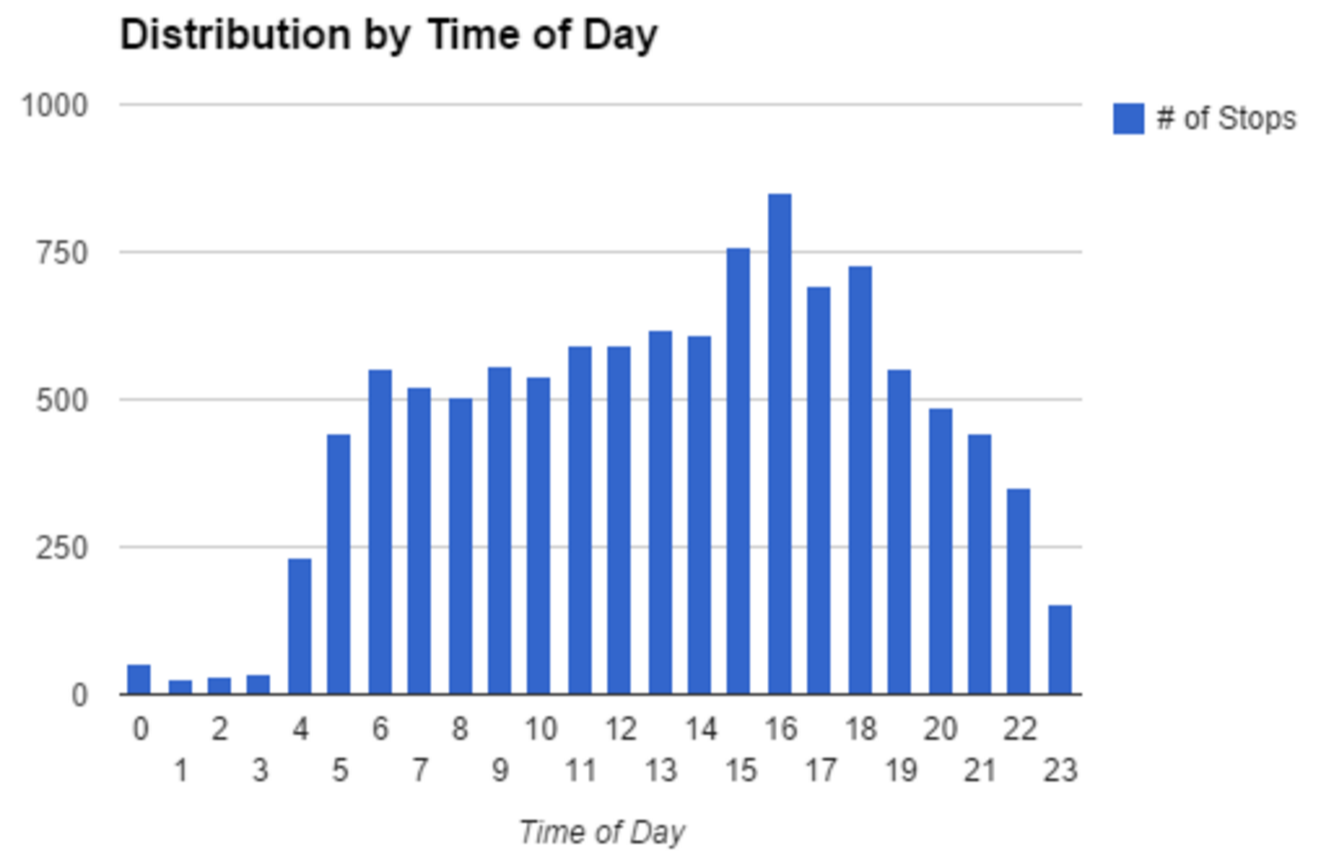
\includegraphics[width=1.0\textwidth]{charts/distribution_time_of_day}
\end{figure}

\begin{figure}[!ht]
	\caption{Distribution by Day of Month}
	\centering
	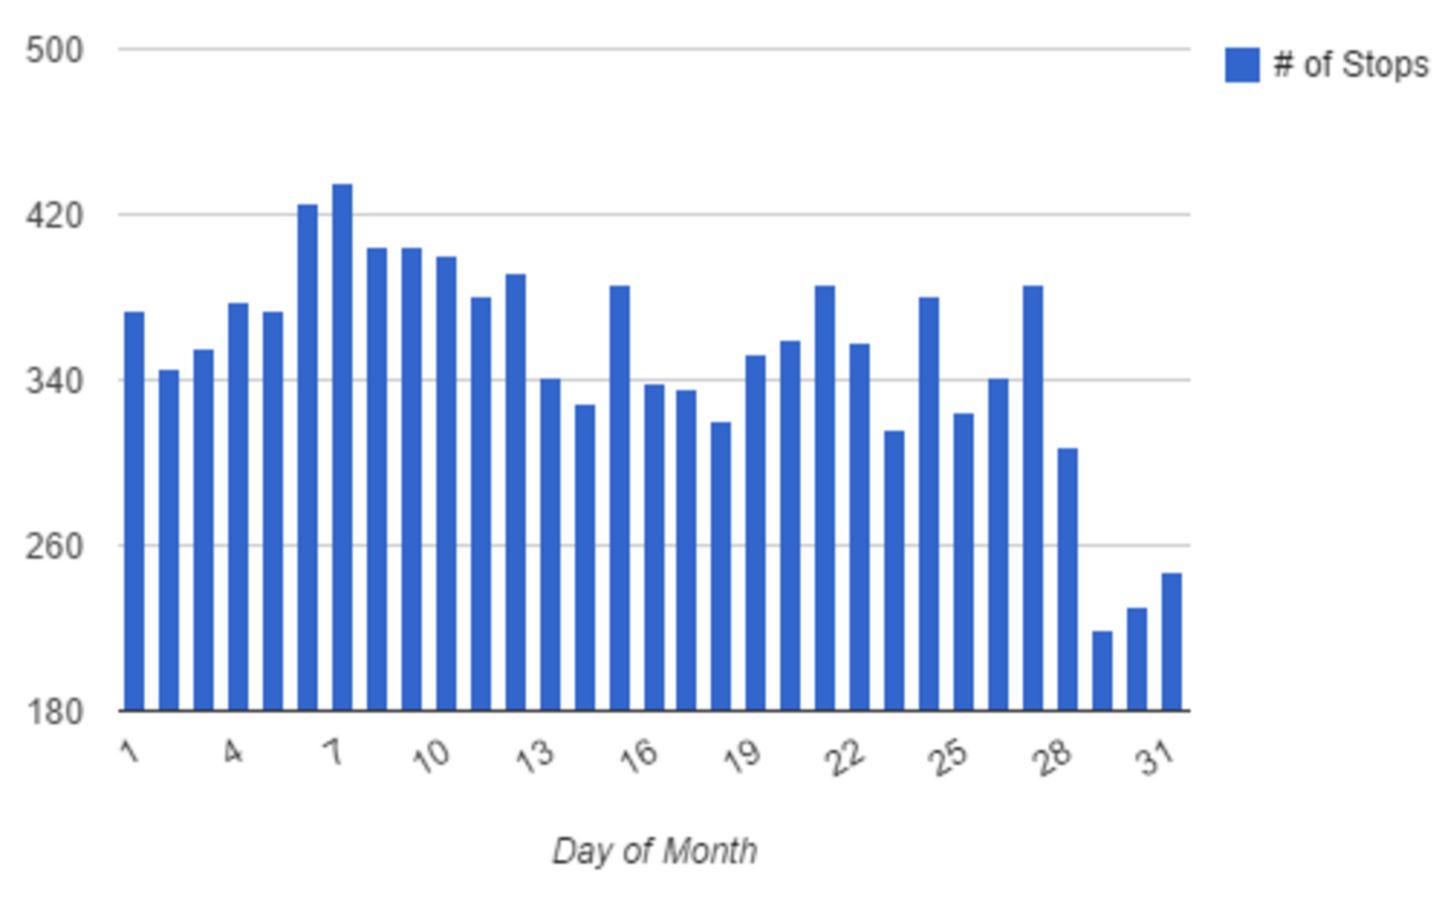
\includegraphics[width=1.0\textwidth]{charts/day_of_month_distribution}
\end{figure}

As we expected we encountered the highest usage during commuting hours, especially in the afternoon. The distribution gets significantly lower as midnight is approached. During the night we have very few gathered data points. The only somewhat surprising point was that the commute hours in the morning didn't produce as high a peak as the hours in the afternoon. However the fact that the data from the app is gathered voluntarily and the app needs to be open to collect data might explain these small inconsistencies.

The distribution by day of month didn't really produce significant insight. The fact that in the end of the month the number of stops are significantly lower is due to fewer months having 31 days. The data set isn't normalized against this and will therefore include such issues. However what this tells us is that the day of month might not be a good indicator. It would be worth exploring the difference between weekday and weekend-day. Since commuting behavior is generally vastly different on weekends as on weekdays this comparison might lead to deeper and more succinct insights.

\begin{figure}[!ht]
	\caption{Number of Stations per User}
	\centering
	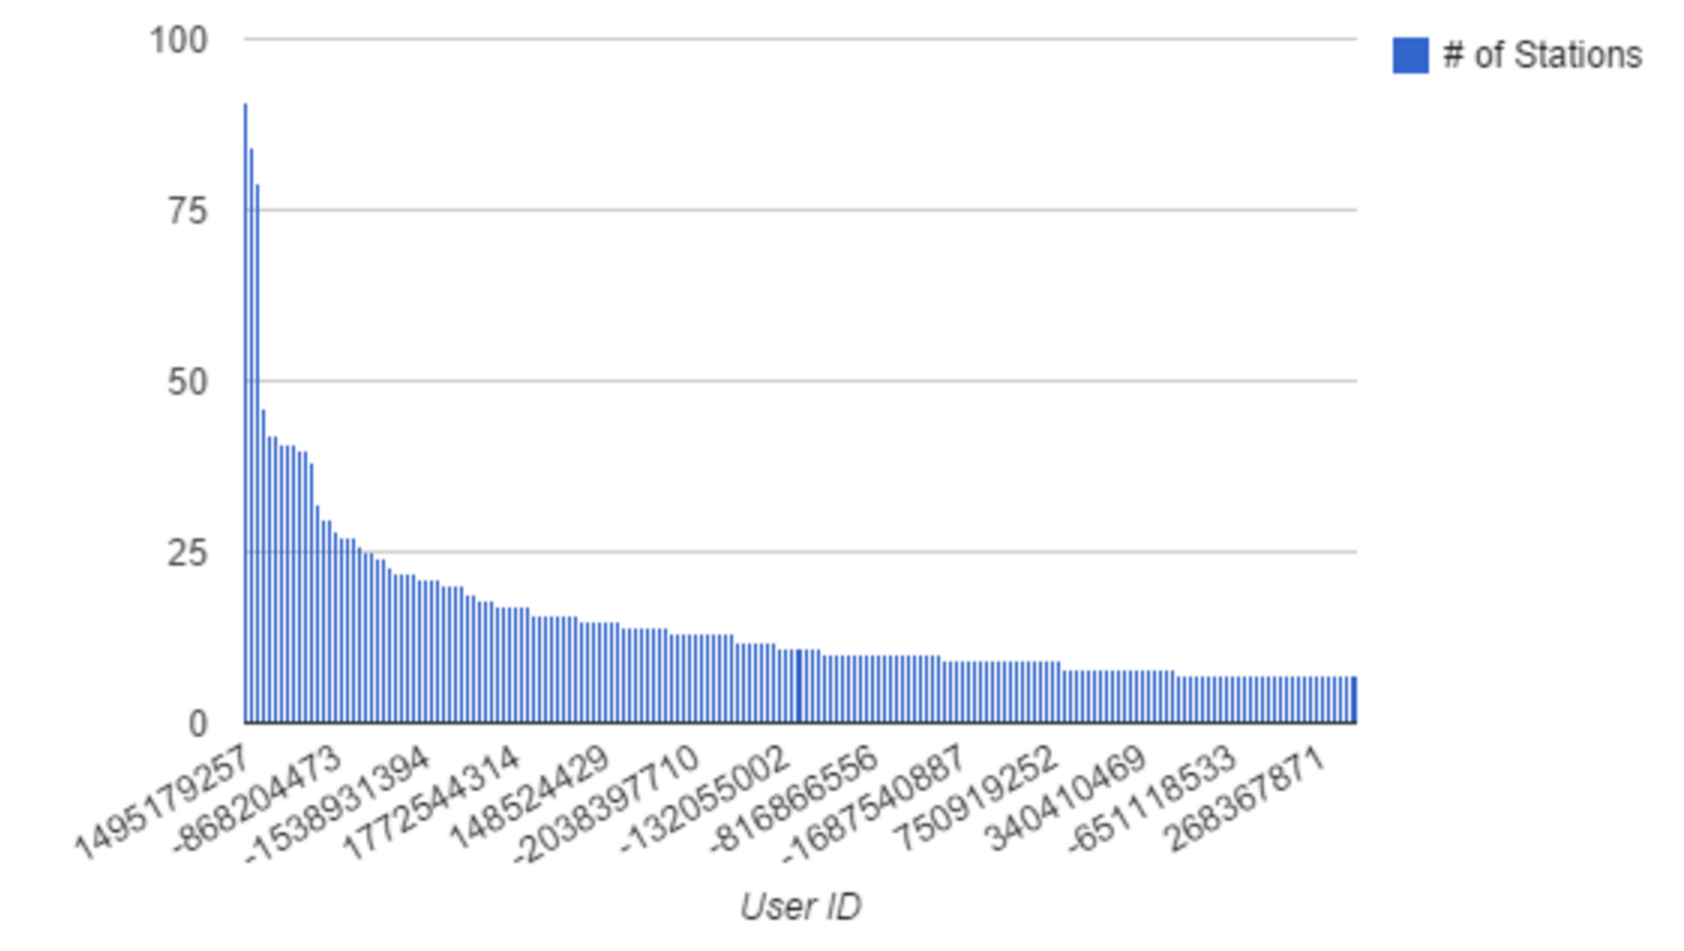
\includegraphics[width=1.0\textwidth]{charts/different_stations_per_user}
\end{figure}


\begin{figure}[!ht]
	\caption{Number of Stops per User}
	\centering
	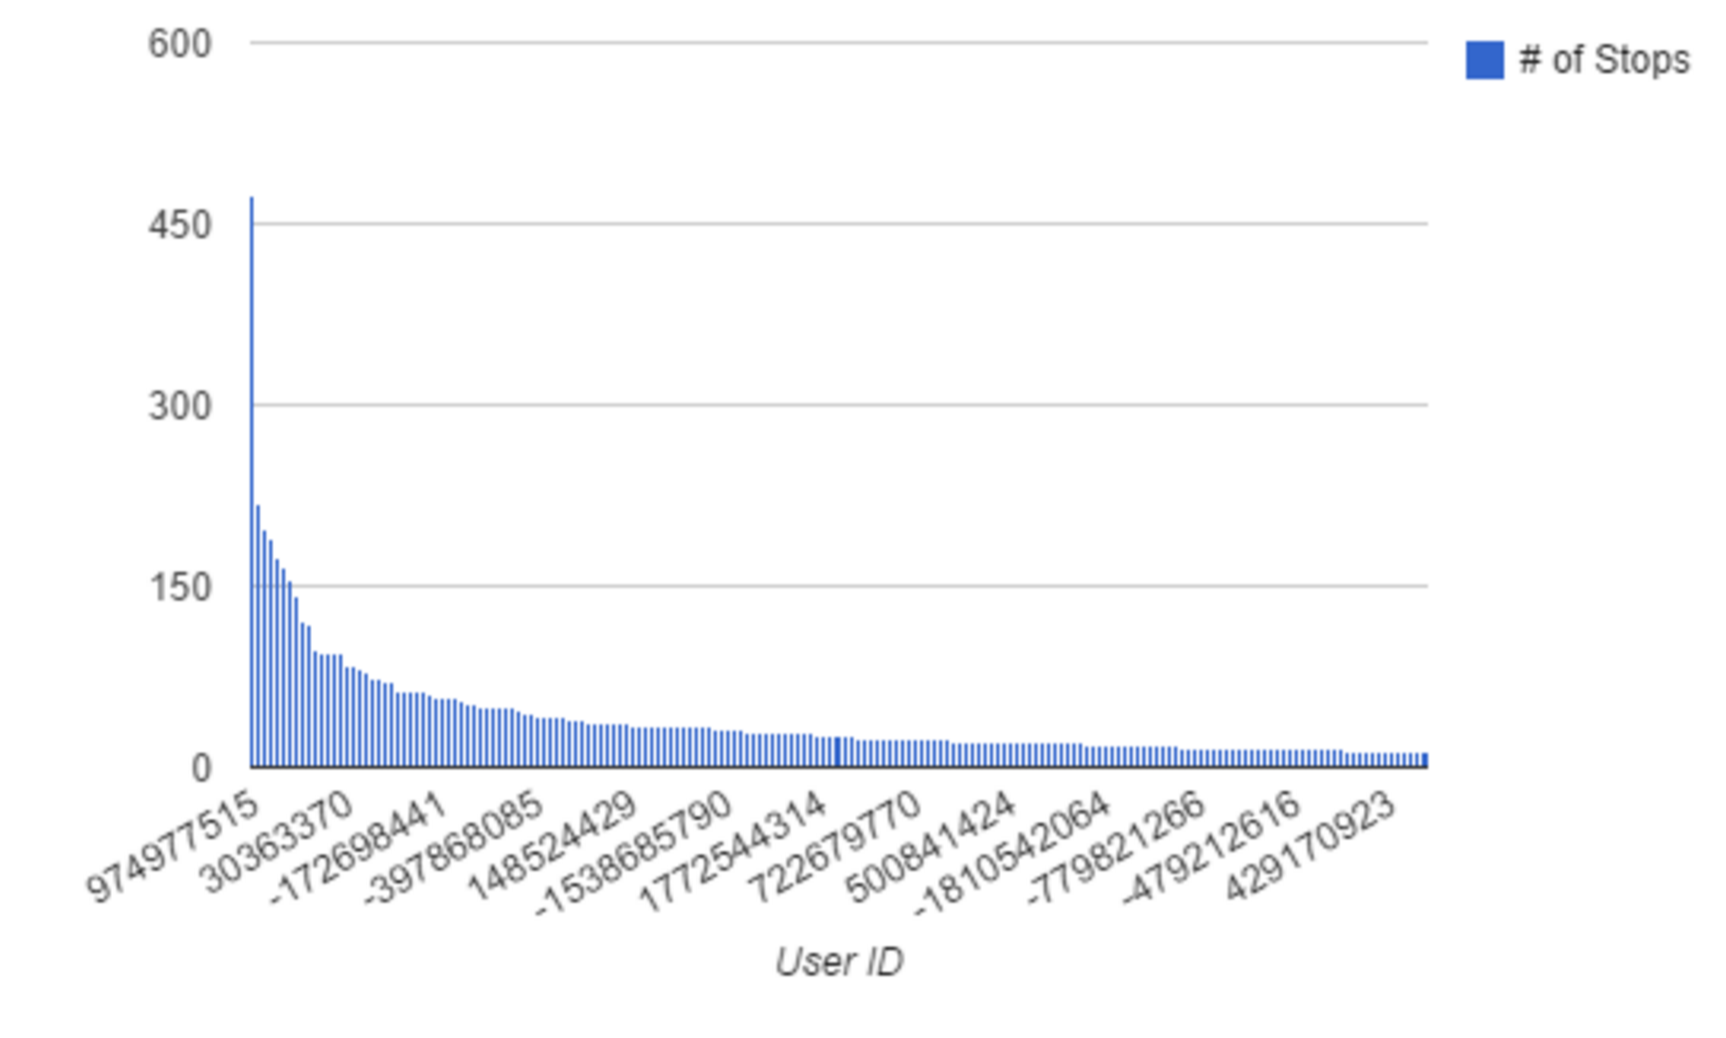
\includegraphics[width=1.0\textwidth]{charts/stops_per_user}
\end{figure}

\begin{figure}[!ht]
	\caption{Number of Users per Station}
	\centering
	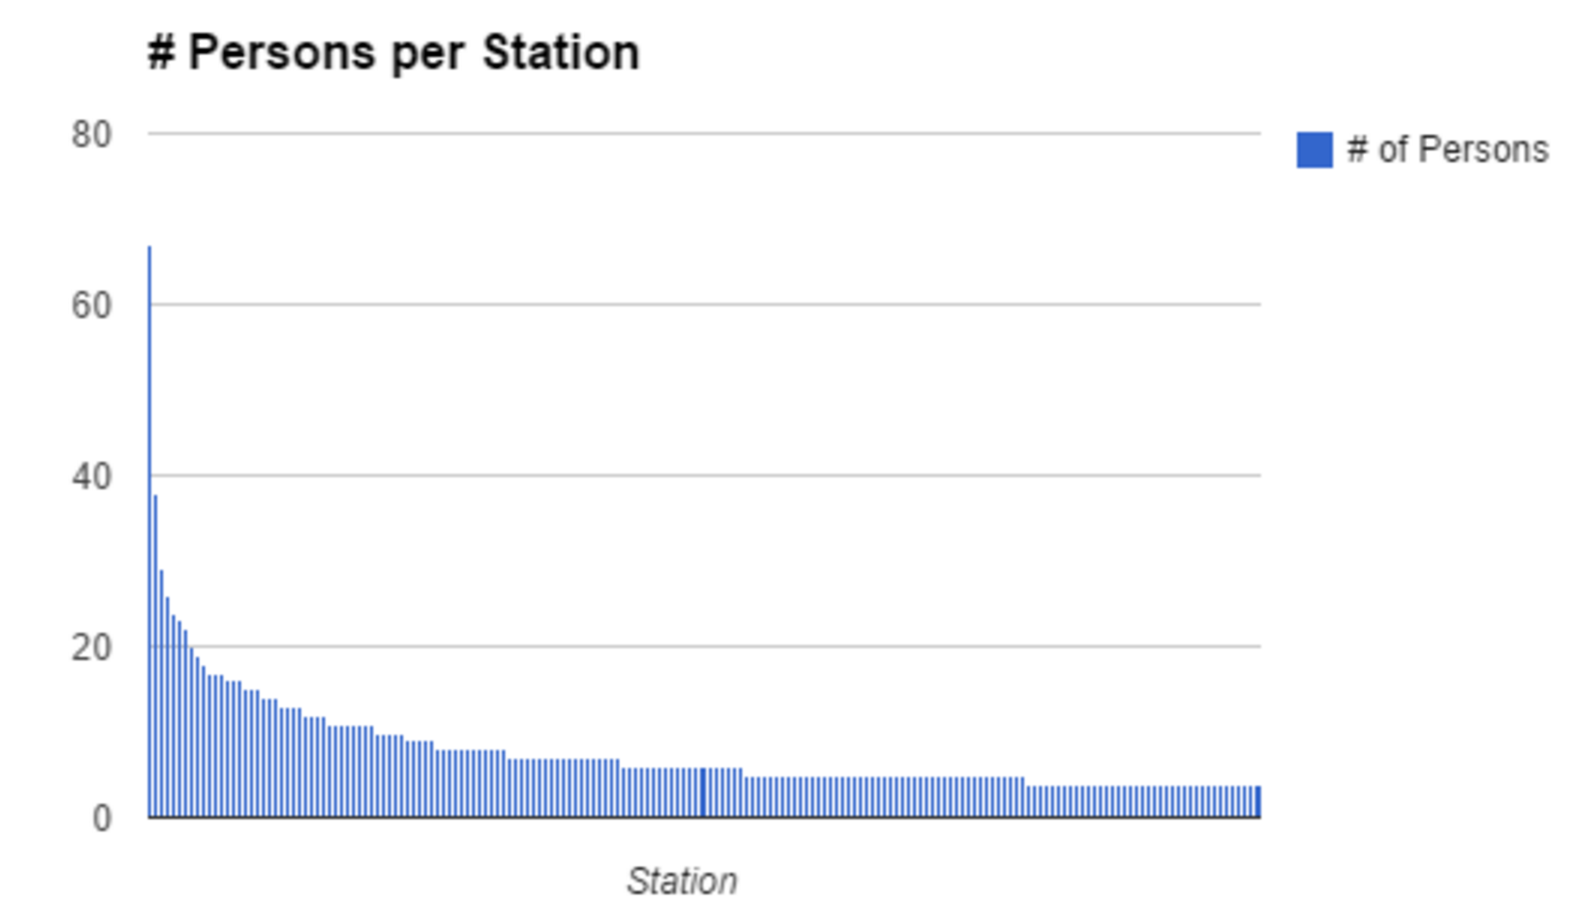
\includegraphics[width=1.0\textwidth]{charts/persons_per_station}
\end{figure}

A vastly more interesting and also challenging conclusion could be drawn from comparing the users with the stations they frequent and how often they stop at stations. As we expected there are a few users that have amassed a lot of data and then there is a long tail of less frequent users. The same statistic also applies to the number of stations and the number of stops that have been gathered for a user. What we already realized here is that it will be very difficult if not impossible to get a good prediction for the users tailing the statistics, simply because there is just not enough data available. In some edge cases where a user really only has 2 or 3 stops that he regularly frequents this might work, otherwise it will just be stabbing in the dark to get a reasonably good prediction. One or two outliers from such a user could possibly mix up the complete prediction process. It seems sensible to cut the dataset into high- and low-frequency users and discard the latter. The exact boundary or whether it will be flexible to a certain degree will have to be tested by trial and error, however if we would not cut the low-frequency user out of our comparison tests it might greatly change our conclusions and the effectiveness of our process.

\begin{figure}[!ht]
	\caption{Distribution of Stops per Station}
	\centering
	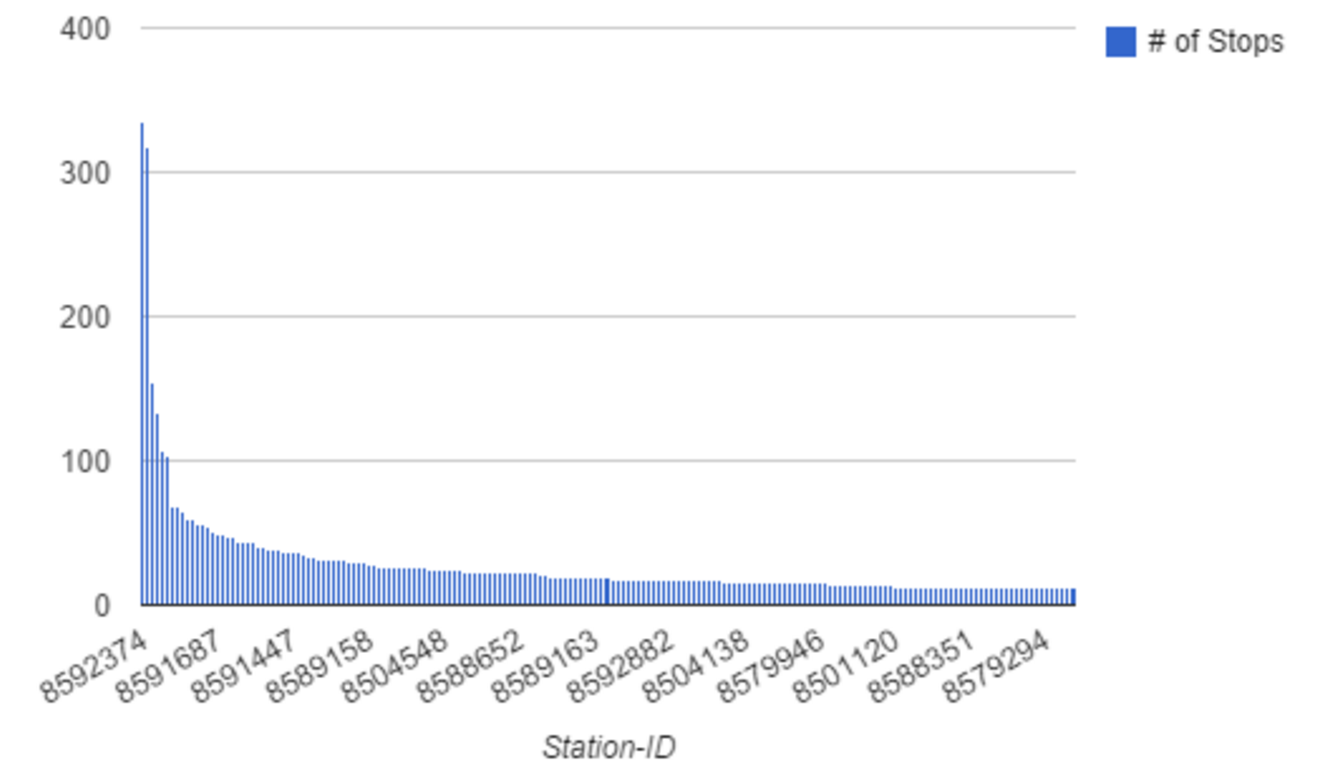
\includegraphics[width=1.0\textwidth]{charts/distribution_stops_by_station}
\end{figure}

\begin{figure}[!ht]
	\caption{Average number of accesses per station by users}
	\centering
	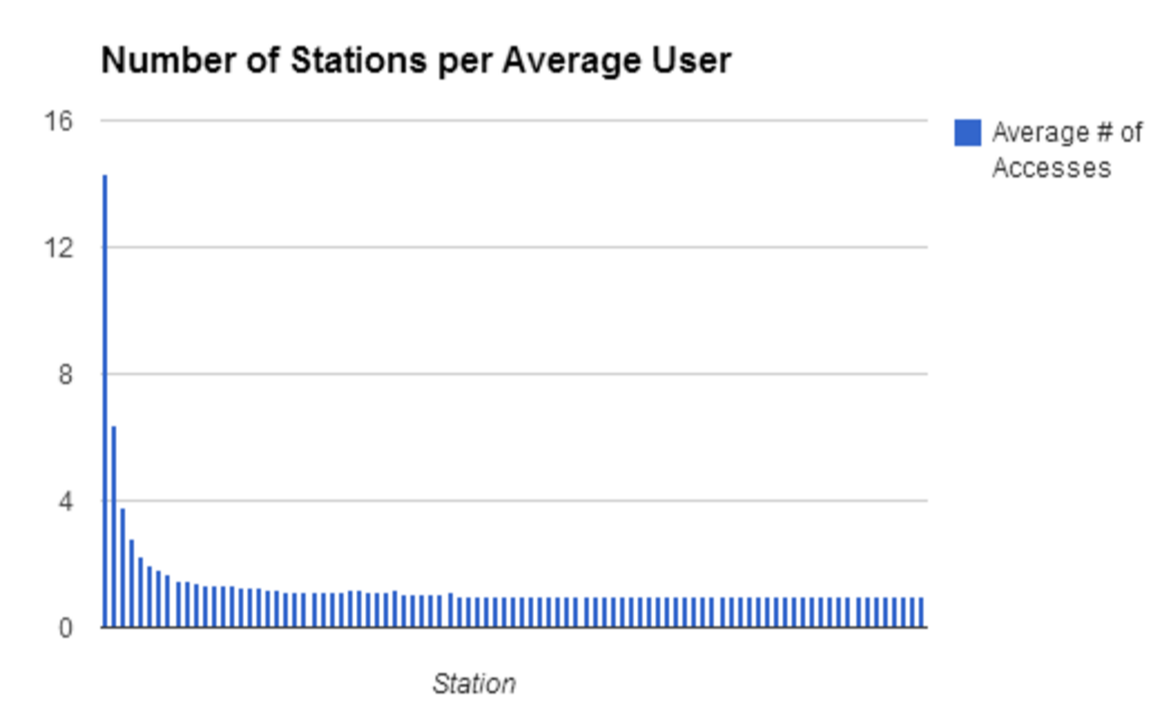
\includegraphics[width=1.0\textwidth]{charts/number_stations_average_user}
\end{figure}

A similar conclusion can also be drawn by the more averaging figures that we created. It also shows a relatively small set with a lot of data and a long, small tail. Combined with the previous conclusions this strengthened our approach of doing statistical analysis and preparing the data set to remove data points that will skew our result. The types of preparation, analysis and restrictions we've imposed on our data set are described in detail in ~\ref{subsubsec:data_preparation}

\subsection{Naive Approach}


\subsection{Machine Learning Results}
\label{subsec:machine_learning_results}

\subsubsection{Execution Plan}
\subsubsection{Data Preparation / Statistical Analysis}
\label{subsubsec:data_preparation}
\subsubsection{Decision Trees (Random Forest is included)}
\subsubsection{Naive Bayes}
\subsubsection{HMM / Neural Networks}

\subsection{Comparison of Results}